

\subsection{Modelos Matem\'aticos \emph{Depredador-Presa}}

El uso de modelos matem\'aticos para describir la din\'amica poblacional de un conjunto de especies que se relacionan mediante interacciones depredador-presa, se remonta a los trabajos de Lotka y Volterra\citep{gotelliprimer}, los cuales independientemente describieron los cambios en la abundancia poblacional de un depredador $C$ y una presa $R$ mediante el siguiente sistema de ecuaciones diferenciales : 

\begin{equation}\label{eq:LV}
\begin{aligned}
&\dot{R} = R(r - \alpha C)\\
&\dot{C} = C(e\alpha - q) 
\end{aligned}
\end{equation}
Donde \emph{r} es la tasa de crecimiento intr\'inseca de la presa $R$, $\alpha$ la tasa de ataque del depredador $C$ y $e$ denota la eficiencia de conversion de individuos consumidos de $R$ a individuos de $C$.\\

El sistema \eqref{eq:LV} es conocido como \emph{sistema de ecuaciones depredador-presa Lotka-Volterra} y se puede extender f\'acilmente a un sistema de $n$ especies indexadas por $\{1,2, \ldots ,n\}$ de la siguiente manera:
\begin{equation}\label{eq:LVGen}
\dot{X_i}  = X_i(b_i - d_i + \sum_{j}^n \alpha_{ij} X_j)
\end{equation}

Donde $X_i$ representa la abundancia en n\'umeros o biomasa de la especie $i$, $b_i$ la tasa intr\'inseca de producci\'on de masa(individuos), $d_i$ la tasa de p\'erdida de masa(individuos) y $\alpha_{ij}$ se puede interpretar como la p\'erdida(ganancia) de masa(individuos) debido a interacciones con las dem\'as especies presentes en el h\'abitat.

Por lo general se asume que :
\begin{itemize}
\item $\alpha_{ij}$ es una constante(la modificaci\'on $\alpha_{ij} = \alpha_{ij}(X)$ para una forma especf\'icia de la funci\'on da lugar a lo que se conoce como respuesta funcional tipo II  o tipo III).
\item $\alpha_{ii} < 0 $ si $X_i$ es un recurso basal, a diferencia de la formulaci\'on original en este caso se asume que existe \emph{denso dependencia directa} entre los individuos de una poblaci\'on de presas.
\item $\alpha_{ii} = 0 $ si $X_i$ es un depredador, es decir no existe \emph{denso dependencia directa} entre individuos de una poblaci\'on de depredadores, sin embargo la denso dependecia se da indirectamente a traves de la interacci\'on con los recursos..
\item $b_i = 0$ si $X_i$ es un depredador, ya que los depredadores no pueden subsistir en ausencia de presas.
\end{itemize}
Modelos como \eqref{eq:LVGen} con los supuestos dados previamente, son llamados \emph{modelos tipo Lotka-Volterra}.

El modelo depredador-presa \emph{Lotka-Volterra}, pese a sus evidentes limitaciones(respuestas funcionales lineales), ha jugado(y sigue jugando) un papel importante en el desarrollo de la teor\'ia en ecolog\'ia y form\'o la base para el desarrollo de modelos que incorporan caracter\'isticas con mayor fundamento biol\'ogico\citep{gotelliprimer,pawar2009community}. \\
Uno de los problemas que surge al momento de construir un modelo similar al de \eqref{eq:LVGen} es el como decidir \emph{a priori} el valor de los par\'ametros del modelo(e.g., $b_i , d_i$). Este problema se hace m\'as notorio conforme la dimensi\'on del modelo(i.e., n\'umero de ecuaciones en el sistema) crece \citep{yodzis1992body}.\\
Yodzis e Innes en su seminal paper \emph{Body size and Consumer-Resource dynamics}\citep{yodzis1992body} propusieron una forma para aligerar el problema. Ellos introdujeron lo que hoy en d\'ia se conoce como \emph{modelamiento bioenerg\'etico} el cual se basa en derivar los valores de los par\'ametros de las relaciones que existen entre ellos y la masa corporal, esta relaci\'on es generalmente de forma indirecta y se manifiesta debido a la influencia que tiene la masa sobre el metabolismo de las especies \citep{peters1986ecological}. A la fecha se han desarrollado diversos refinamientos a estas ideas, lo cual nos permite centrarnos en par\'ametros con mayor significado biol\'ogico \citep{kiltie2000scaling,brown2004toward,savage2004predominance,pawar2012dimensionality,brose2010body}.

\subsection{Ensamblaje}
En esta secci\'on definimos ciertos t\'erminos relacionados al proceso de ensamblaje de una comunidad. \\
Se denomina proceso de ensamblaje $E_A$ de una comunidad $A$ asociada a un h\'abitat $H$ al continuo de colonizaciones y extinciones de especies que se dan dentro de $H$(los cuales a su vez modifican $H$), el conjunto de especies que \emph{potencialmente} puede colonizar a la comunidad $A$(i.e pueden por lo menos llegar a $H$) se denomina \emph{pool regional de especies}. 
\begin{equation}\label{eq:Assembly}
E_A := (A_0,H_0) \to (A_1,H_1) \to (A_2,H_2) \to \ldots
\end{equation}

En \eqref{eq:Assembly} cada cambio de $(A_i,H_i)$ a $(A_{i+1},H_{i+1})$ se da debido a un intento de colonizaci\'on sobre $(A_i,H_i)$,el cual puede tener uno de los tres siguientes desenlaces \citep{pawar2009community}: 
\begin{enumerate}
\item El invasor no puede invadir.
\item El invasor llega a invadir pero provoca extinciones en la comunidad receptora, pudiendo el mismo exintiguirse, esto es llamado \emph{invasi\'on inestable}.
\item El invasor llega a invadir y no provoca ninguna extinci\'on, esto es llamado \emph{invasi\'on estable}.
\end{enumerate}

De lo anterior se observa que la comunidad y el h\'abitat f\'isico receptor juegan un papel muy importante en el subsiguiente paso del proceso, adem\'as especificamos que cada estado $(A_i,H_i)$ puede estar en constante cambio,excepto por el n\'umero de especies, debido a la din\'amica inherente de las poblaciones de las especies presentes; y por ende el tiempo entre distintas colonizaciones puede influenciar el desenlace de la colonizaci\'on, debido a que la comunidad receptora puede estar en distintos estados(e.g., estado transiente $vs$ estado asint\'otico).\\

Sea $B = \{ (A_j,H_j) / j \in I, I \subseteq \mathbb{N}\}$ un conjunto de estados en $E_A$ , usando el formalismo definido en \eqref{eq:Assembly} decimos que la comunidad $A$ \emph{$\omega$-converge} a $B$ durante el ensamblaje si existe un $ m \in \mathbb{N}$ tal que $(A_i,H_i) \in B, i \geq m$. Sea $D$ el menor de los conjuntos(respecto a la inclusi\'on) a los cuales la comunidad $A$ $\omega-converge$. Decimos entonces que la comunidad $A$ \emph{converge} a $D$.

\subsubsection{Caminos de Ensamblaje}
Sea $\hat{A}$ un conjunto de especies con un set de interacciones $S$ y un habitat $\hat{H}$, una secuencia de colonizaciones $\mathcal{C}$ tal que el estado final es $(\hat{A},S,\hat{H})$ es llamado \emph{camino de ensamblaje} hacia $(\hat{A},S,\hat{H})$.

\subsection{ M\'odulo IGP}

En teor\'ia de redes tr\'oficas, se denomina \emph{m\'odulos comunitarios} a un conjunto peque\~no de especies que interact\'uan entre s\'i y cuyo patr\'on de interacci\'on ha sido encontrado en diversos ecosistemas \citep{holt1997community}. Entre ellos el m\'odulo de \emph{depredaci\'on dentro del clan}(IGP por sus siglas en ingl\'es), el cual fue descrito por primera vez por \cite{polis1989ecology}, envuelve tres especies: un recurso basal, un depredador intermedio y un depredador tope. Ambos depredadores consumen al recurso y ademas el depredador intermedio es consumido por el depredador tope. Este sistema pese a tener solo $3$ especies incorpora diversos tipos de interacci\'on \emph{depredaci\'on, competencia aparente, competencia por explotaci\'on y mutualismo indirecto}. Esto se describe gr\'aficamente en la figura \ref{fig:IGP}
\begin{figure}[h]
\begin{tikzpicture}[<->,>=stealth',shorten >=1pt,auto,
  thick,main node/.style={circle,fill=blue!20,draw,font=\sffamily\Large\bfseries}]


\node[main node] (R) at (0,-3){R};
\node[main node] (C) at (3,0) {C};
\node[main node] (P) at (0,3) {P};

 \path[every node/.style={font=\sffamily\small}]

(R) edge [<-,red] (C)
(R) edge [<-,red] (P)
(P) edge [->,red] (C)
(P) edge [bend right , dotted, blue] (R) 
(P) edge [bend left , dotted, green]  (C)
(R) edge [bend right ,dotted , black] (C);



\begin{customlegend}[legend cell align=left,
legend entries={ % <= in the following there are the entries
Depredaci\'on,
Competencia por explotaci\'on,
Competencia aparente, 
Mutualismo indirecto
},
legend style={at={(-1.5,3.5)},font=\footnotesize}] % <= to define position and font legend
% the following are the "images" and numbers in the legend
    \addlegendimage{-stealth,red}
    \addlegendimage{stealth-stealth,dotted,green}
    \addlegendimage{stealth-stealth,dotted,black}
    \addlegendimage{stealth-stealth,dotted,blue}
    
\end{customlegend}

\end{tikzpicture}

\caption{M\'odulo \textbf{IGP}}
\label{fig:IGP}
\end{figure}

Adem\'as este sistema es el menor(en el sentido de n\'umero de especies) en el cual podemos encontrar 2 \emph{caminos de ensamblaje} (figura \ref{fig:IGPAssembly}).
\begin{figure}[h]
\begin{center}
\begin{tikzpicture}[->,>=stealth',shorten >=1pt,auto,
  thick,main node/.style={circle,fill=blue!20,draw,font=\sffamily\Large\bfseries}]

\node[main node](R1) at (1,0) { R};
\node[main node](C1) at (0,2) {C};
\node[main node](C2) at  (4,2){C};
\node[main node](R2) at ($(R1) + (3,0)$) {R};
\node[main node](P1) at (5,4){P};
\node[main node](R3) at ($(R2) + (3,0)$){R};
\node[main node](C3) at ($(R3) + (1,2)$){C};
\node[main node](P3) at ($(R3) + (0,4)$){P};
\node[font = \fontsize{15}{15}\selectfont](A1) at (-4,0) {Camino 1};

\path
(C1) edge[bend left,dotted] (R1)
($(R1)+(1.0,0)$) edge[line width = 2]  ($(R1)+ (2,0)$)
(R2) edge (C2)
(P1) edge[bend right,dotted] (C2)
(P1) edge[bend left,dotted] (R2)
($(R2) + (1.0,0)$) edge[line width  = 2] ($(R2) + (2,0)$)
(R3) edge (C3)
(R3) edge (P3)
(C3) edge (P3);
\end{tikzpicture}
$\left. \right.$\\
$\left. \right.$\\

\begin{tikzpicture}[->,>=stealth',shorten >=1pt,auto,
  thick,main node/.style={circle,fill=blue!20,draw,font=\sffamily\Large\bfseries}]

\node[main node](R1) at (1,0) { R};
\node[main node](P1) at (0,2) {P};
\node[main node](P2) at  (4,4){P};
\node[main node](R2) at ($(R1) + (3,0)$) {R};
\node[main node](C1) at (5,2){C};
\node[main node](R3) at ($(R2) + (3,0)$){R};
\node[main node](C3) at ($(R3) + (1,2)$){C};
\node[main node](P3) at ($(R3) + (0,4)$){P};
\node[font = \fontsize{15}{15}\selectfont](A1) at (-4,0) {Camino 2};

\path
(P1) edge[bend left,dotted] (R1)
($(R1)+(1.0,0)$) edge[line width = 2]  ($(R1)+ (2,0)$)
(R2) edge (P2)
(C1) edge[bend left,dotted] (R2)
(P2) edge[bend left,dotted,red] (C1)
($(R2) + (1.0,0)$) edge[line width  = 2] ($(R2) + (2,0)$)
(R3) edge (C3)
(R3) edge (P3)
(C3) edge (P3);

\end{tikzpicture}
\end{center}

\caption{\emph{Caminos de ensamblaje} para el m\'odulo \textbf{IGP}, denotamos $S_1$ al camino superior y $S_2$ al inferior}
\label{fig:IGPAssembly}
\end{figure}
Numerosos ejemplos son citados en \cite{polis1989ecology,arim2004intraguild}

\subsection{Distribuci\'on de Masas}
Una distribuci\'on de masas en una comunidad $C$ es la imagen de una funci\'on  $f : C \to \mathbb{R}$ donde a cada conjunto de individuos de una especie $S$ se le asocia la masa promedio $m_S$ encontrada en $S$. Una distribuci\'on de masas proveniente de una recolecci\'on emp\'irica se representa gr\'aficamente mediante histogramas. \\
Generalmente la forma de la distribuci\'on se considera una caracter\'istica de la comunidad, y se ha demostrado que influencia la distribuci\'on de autovalores y otras propiedades din\'amicas de ella.\\

En el m\'odulo IGP dado que solo esta compuesto de tres especies podemos describir la distribuci\'on de las masas presente mediante las relaciones que existen entres las masas de las tres especies y distinguir estos 6 tipos de comunidades :
\begin{enumerate}
  \item $m_P > m_C > m_R$
  \item $m_P > m_R > m_C$
  \item $m_R > m_C > m_P$
  \item $m_R > m_P > m_C$
  \item $m_C > m_P > m_R$
  \item $m_C > m_R > m_P$
\end{enumerate}

Estas relaciones entre masas son equivalentes a relaciones entre las razones de masas presentes en el m\'odulo. 
Definimos :
\begin{equation}\label{eq:SR}
  \begin{aligned}
    &k_{\RC} \equiv \frac{m_R}{m_C}\\
    &k_{\CP} \equiv \frac{m_C}{m_P}\\
    &k_{\RP} \equiv \frac{m_R}{m_P} = k_{\RC} k_{\CP}
  \end{aligned}
\end{equation}

Podemos designar cada comunidad por su particular relaci\'on de masas :
\begin{enumerate}[label=(\alph*)]
\item $\mathbf{C}_1$ sss $k_{\RC} \leq 1 , k_{\RP} \leq 1 ,k_{\CP} \leq 1$
\item $\mathbf{C}_2$ sss $k_{\RC} > 1 , k_{\RP} \leq 1 ,k_{\CP} \leq 1$
\item $\mathbf{C}_3$ sss $k_{\RC} > 1 , k_{\RP} > 1 ,k_{\CP} \leq 1$
\item $\mathbf{C}_4$ sss $k_{\RC} > 1 , k_{\RP} > 1 ,k_{\CP} > 1$
\item $\mathbf{C}_5$ sss $k_{\RC} \leq 1 , k_{\RP} > 1 ,k_{\CP} > 1$
\item $\mathbf{C}_6$ sss $k_{\RC} \leq 1 , k_{\RP} \leq 1 ,k_{\CP} > 1$
\end{enumerate}

Bajo este criterio podemos seccionar el espacio $k_{\CP} \times k_{\RC}$ en 6 zonas. Esto se represta gr\'aficamente en la figura ~\ref{fig:ZonasSR}

\begin{figure}[h!]
  \centering
  \begin{tikzpicture}[<->,>=stealth',shorten >=0.1pt,auto,
  thick,main node/.style={circle,fill=blue!20,draw,font=\sffamily\Large\bfseries}]


\node (fig1) at (-3,-5)
       {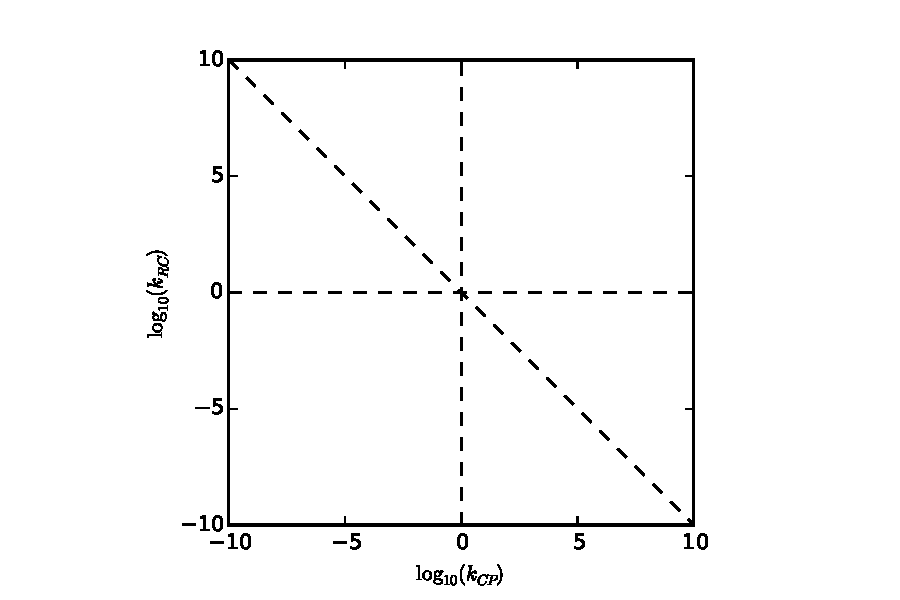
\includegraphics[scale=0.8]{C:/Users/Carlos/Documents/Tesis-IGP/code/Theory/ZonesSR.pdf}};

\node[circle,fill= blue!20,draw, minimum size=0.6cm,inner sep= 0] (R) at (-5.5,-4.5){R};
\node[circle,fill=blue!20,draw,minimum size=0.3cm, inner sep = 0] (C) at (-4.5,-3.8) {C};
\node[circle,fill=blue!20,draw,minimum size=1.cm,inner sep = 0](P) at (-5.5,-3.) {P};

 \path[every node/.style={font=\sffamily\small}]

(R) edge [<-,red] (C)
(R) edge [<-,red] (P)
(P) edge [->,red] (C);


\node[circle,fill= blue!20,draw, minimum size=0.3cm,inner sep= 0] (R) at (-4.5,-7.8){R};
\node[circle,fill=blue!20,draw,minimum size=0.6cm, inner sep = 0] (C) at (-3.5,-6.7) {C};
\node[circle,fill=blue!20,draw,minimum size=1.cm,inner sep = 0](P) at (-4.5,-5.6) {P};

 \path[every node/.style={font=\sffamily\small}]

(R) edge [<-,red] (C)
(R) edge [<-,red] (P)
(P) edge [->,red] (C);


\node[circle,fill= blue!20,draw, minimum size=1.cm,inner sep= 0] (R) at (-3.4,-3.6){R};
\node[circle,fill=blue!20,draw,minimum size=0.3cm, inner sep = 0] (C) at (-4.3,-2.6) {C};
\node[circle,fill=blue!20,draw,minimum size=0.6cm,inner sep = 0](P) at (-3.4,-2.1) {P};

 \path[every node/.style={font=\sffamily\small}]

(R) edge [<-,red] (C)
(R) edge [<-,red] (P)
(P) edge [->,red] (C);



\node[circle,fill= blue!20,draw, minimum size=1.cm,inner sep= 0] (R) at (-1.5,-4.1){R};
\node[circle,fill=blue!20,draw,minimum size=0.6cm, inner sep = 0] (C) at (-0.3,-3) {C};
\node[circle,fill=blue!20,draw,minimum size=0.3cm,inner sep = 0](P) at (-1.5,-2.1) {P};

 \path[every node/.style={font=\sffamily\small}]

(R) edge [<-,red] (C)
(R) edge [<-,red] (P)
(P) edge [->,red] (C);


\node[circle,fill= blue!20,draw, minimum size=0.6cm,inner sep= 0] (R) at (-0.1,-7){R};
\node[circle,fill=blue!20,draw,minimum size=1.0cm, inner sep = 0] (C) at (-1,-5.9) {C};
\node[circle,fill=blue!20,draw,minimum size=0.3cm,inner sep = 0](P) at (-0.1,-5.2) {P};

 \path[every node/.style={font=\sffamily\small}]

(R) edge [<-,red] (C)
(R) edge [<-,red] (P)
(P) edge [->,red] (C);


\node[circle,fill= blue!20,draw, minimum size=0.3cm,inner sep= 0] (R) at (-2.55,-7.8){R};
\node[circle,fill=blue!20,draw,minimum size=1.cm, inner sep = 0] (C) at (-1.8,-6.7) {C};
\node[circle,fill=blue!20,draw,minimum size=0.6cm,inner sep = 0](P) at (-2.55,-5.7) {P};

 \path[every node/.style={font=\sffamily\small}]

(R) edge [<-,red] (C)
(R) edge [<-,red] (P)
(P) edge [->,red] (C);


   
\end{tikzpicture}

  \caption{Divisi\'on del espacio $k_{\CP} \times k_{\RC}$ en funci\'on ah las relaciones de orden existentes entre las masas de las tres especies.}
\label{fig:ZonasSR}
\end{figure}
  
\subsection{Longitud de Cadenas tr\'oficas}

Si bien existen distintas formas de medir la longitud de las cadenas tr\'oficas \citep{post2002long} en este trabajo usaremos el concepto de \emph{posici\'on tr\'ofica} de una especie \citep{TP2007proximate}, el cual esta definido como :
\begin{equation}
TP_j = \sum_{i \in G} (1+TP_i) p_i 
\end{equation}
Donde $G$ es el conjunto de presas del predador $j$ y $p_i$ es la proporci\'on de energ\'ia y materia derivada de la consumci\'on de la presa $i$. A nivel comunitario se reporta la m\'axima posici\'on tr\'ofica que se puede interpretar como la \emph{altura} de la red tr\'ofica en la cual estan embebidas todas las interacciones \emph{depredador-presa} de la comunidad.\\
El concepto de m\'axima posici\'on tr\'ofica es adecuado para tratar el hecho que en la naturaleza existe un gran nivel de omnivorismo \citep{arim2004intraguild,williams2004limits,thompson2007trophic}, y por ende no se espera la presencia de cadenas lineares, sino que todas estas interacciones estan embebidas en una estructura reticular .

\subsection{Hip\'otesis asociadas a FCL}

La b\'usqueda de los determinantes de la longitud de las cadenas tr\'oficas se remonta a la pregunta hecha por Elton(1927) : �Qu\'e limita la longitud de las cadenas tr\'oficas?, esto debido a que emp\'iricamente se estaba encontrando cadenas no mayores de 5 pasos, numerosos estudios se han conducido desde entonces, emergiendo diversas hip\'otesis, las cuales ser\'an citadas a continuaci\'on acompa\~nadas de sus respectivos proponentes.\\
\begin{enumerate}[label=(\alph*)]

\item \textbf{Limitaciones energ\'eticas}: Propuesta por \citet{lindeman1942trophic}, extendida por \citet{hutchinson1959homage} y \citet{schoener1989food}, este \'ultimo consider\'o al espacio expl\'icitamente. Siendo esto una simple adaptaci\'on de la segunda ley de la termodin\'amica y en la cual se propone que la longitud est\'a limitada debido a que la transferencia de energ\'ia no es perfecta de manera tal que a trav\'es de cada nivel tr\'ofico se va perdiendo parte de la energ\'ia producida por el nivel tr\'ofico previo, por lo que conforme aumenta el n\'umero de niveles tr\'oficos la energ\'ia disponible hacia el nivel tr\'ofico superior(si existiera) es cada vez menor. La validaci\'on emp\'irica se basa en evaluar la correlaci\'on entre el nivel de productividad del h\'abitat y la m\'axima FCL \citep{kaunzinger1998productivity,wootton1993productivity}, si bien el nivel de productividad basal a niveles muy bajos siempre ser\'ia un limitante de FCL,dado que para que al menos un nivel persista se necesita que haya un nivel de energ\'ia y materia m\'inimo(el cual depender\'a de la especie en consideraci\'on), su influencia en casos no tan extremos ha sido cuestionada (\citet{post2000ecosystem},v\'ease sin embargo \citet{young2013roles}). Un argumento que usa el concepto de \emph{centripetality} asociado a proceso autocatal\'iticos ha sido postulada por \citet{ulanowicz2014limits}, el cual sin embargo se reduce a una consecuencia de la segunda ley de la termodin\'amica, con la diferencia de que su accionar no es uniforme para distintos niveles de organizaci\'on del sistema.

\item \textbf{Estabilidad din\'amica}: Postulada por \citet{pimm1978feeding} , donde te\'oricamente demostraron que una cadena m\'as larga era m\'as inestable( medida de estabilidad de acuerdo al tiempo de vuelta hacia el estado de equilibrio) y por ende tendr\'ia una menor probabilidad de ser observada.Sin embargo \citet{sterner1997enigma} han refutado esta idea, haciendo ver que lo que supuestamente encontraron Pimm y Lawton era dependiente de los factores de regulaci\'on presentes en el sistema(e.g., denso-dependencia intraespec\'ifica), lo cual Pimm y Lawton incorporaron solo a nivel basal, si se controlan los factores a medida que uno alarga la cadena, en contradicci\'on con lo originalmente postulado, las cadenas se vuelven m\'as estables(Sterner et al. 1997). El trabajo de \citet{borrelli2014there} reafirma la observaci\'on inicial encontrando en la mayor\'ia de los casos una relaci\'on negativa entre la m\'axima FCL y la estabilidad del sistema, medido en base al criterio de \emph{Quasi-sign stability}\citep{allesina2008network}. Esta hip\'otesis se ha medido empiricamente viendo la correlaci\'on entre el r\'egimen de disturbancia del ambiente y la m\'axima FCL encontrandose efectos significativos en algunos casos y nulos en otros\citep{takimoto2008ecosystem,power1996disturbance}.

\item \textbf{Tama\~no del ecosistema}: Postulada entre otros por \citet{cohen1991community} y \citet{post2000ecosystem}, donde sugieren que el tama\~no del ecosistema es el responsable de la longitud observada en las cadenas tr\'oficas, relacionada con las ideas de curva especie-\'area, i.e mayor \'area implica mayor n\'umero de especies lo que potencialmente da lugar a una cadena tr\'ofica m\'as larga \citep{holt2002food,holt1999trophic}, como tambi\'en sugiriendo el hecho que una mayor \'area aminora las inestabilidades din\'amicas  que puede tener un sistema limitado espacialmente\citep{holt2002food,mccann2005dynamics} esta hip\'otesis ha sido validad emp\'iricamente en distintos ambientes \citep{post2000ecosystem,takimoto2008ecosystem}, sin embargo igual que en los dos casos anteriores existen reportes donde este factor no es un buen predictor de la m\'axima FCL \citep{young2013roles}

\item \textbf{Din\'amica adaptativa}: Un trabajo reciente de \citet{kondoh2009food} rejuvenecen la idea de \citet{hastings1979length} proponiendo que la din\'amica adaptativa del depredador al momento de elegir a su presa es un factor clave en la limitaci\'on de la longitud de las cadenas tr\'oficas.
\end{enumerate}

A pesar de la gran cantidad de trabajos realizados en este tema, no hay a\'un una conclusi\'on definitva, debido a lo cual Takimoto y Post(2012) sugieren que, con la teor\'ia actual a\'un no se pueden entender algunos patrones observados en la naturaleza.












